% !TEX root = CartaPerali_Report.tex
\section{Processing Pipeline}
\label{sec:processing_pipeine}

\noindent The code necessary to replicate this work is available in the GitHub repository \footnote{https://github.com/Fisher4537/HumanDataAnalitycs}.\\
The workflow used to implement the whole KWS system is depicted in Fig. \ref{fig:pipeline}.
\begin{figure}[h]
			\centering
	    	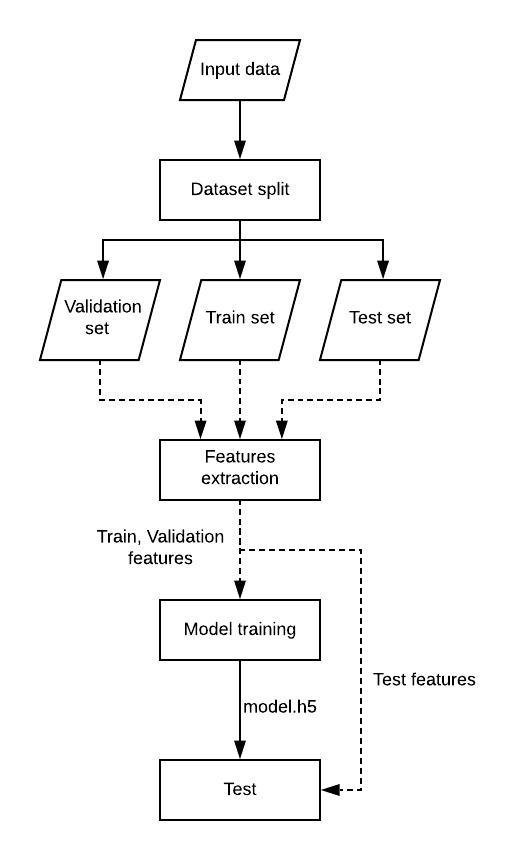
\includegraphics[width=6cm, height=8cm ,width=0.25\textwidth]{pipeline}
	    	\caption{System workflow}
	    	\label{fig:pipeline}
\end{figure} 
\noindent As mentioned in the intro, the input data are downloaded from the well known public '{\it{speech\_commands}}' dataset \cite{Warden-2018}. At the time of this project it counts 105829 \textit{wav}, 16000 Hz, channel mono audio files. Each of them is listed and the file dimension is checked: only the file with size of 32K are kept, the other are discarded, indeed the audio with length less than 1 s have an higher probability to contain truncated word spell. \\
As suggested by the author of the dataset \cite{Warden-2018}, to split the it into \textit{train}, \textit{validation} and \textit{test}, the hash of each audio is used to avoid that two different audio with the same label and pronounced by the same person would be put on different set (see \textit{which\_set} method described by the author in the README), compromising the interdependence between the different sets. \\
The dataset is too huge be loaded into conventional RAM, therefore each list (train, validation and test) is dynamically split into lighter batches by specific generator (represented as dashed line in fig. \ref{fig:pipeline}). Each generator return a preprocessed audio as described next, which is consumed during the train and/or test phase.\\
\textbf{Balanced batches and unknown percentage.} In a real application an audio stream is full of background noise and utterance to ignore. The keywords to recognize are only a little part. To differentiate background noise and unknown utterance, an \textit{unknown} label is added to the wanted words. The \textit{unknown} class should be composed of audio depending of the application context. In this report the problem is not faced. However it is provided a simple mechanism for the management of unknown label and the percentage of each label of the dataset. A list of \textit{wanted words} is passed as input parameter with an unknown percentage value. Each returned batch has the specified percentage of unknown audios taken from the file which are not in the wanted word list. In the report, each dataset with a specific percentage of unknown is defined as \textit{balanced}, instead, \textit{unbalanced} dataset has no specific unknown percentage and that class composed of all the speech recognition audio that are not labeled with a specified wanted word.


\section{Data preprocessing and Features extraction}
\label{sec:model}

\noindent Data are preprocessed by \textit{generators} that are responsible for preparing batches of data containing the desired percentage of predefined wanted words, organized in a list, and the percentage of words that the model should classify as \textit{unknown}. \\
Two different type of input are considered in this report: Mel-Frequency Cepstrum Coefficients or the spectrogram of the input file. MFCC is obtained with an external library "python\_speech\_command", and represent ...  MFCC frames are built using parameters depicted in Table \ref{table:mfcc_parameters}.
\begin{table}[h!]
	\centering
	\begin{tabular}{ p{3cm}|p{3cm}|}
		\hline
		Window length & 25ms \\
		Frame shift  & 10ms  \\
		N. Filterbanks & 26\\
		N. FFT points & 512\\
		\hline
	\end{tabular}
	\caption{MFCC parameters}
	\label{table:mfcc_parameters}
\end{table}
\noindent In the end, one set of 13 MFCC coefficients is extracted from each frame. 
The spectrogram is obtained by applying fast fourier transform to overlying subsequent intervals of the input audio and it represent the active frequency over the time.


\begin{figure}
	\centering
	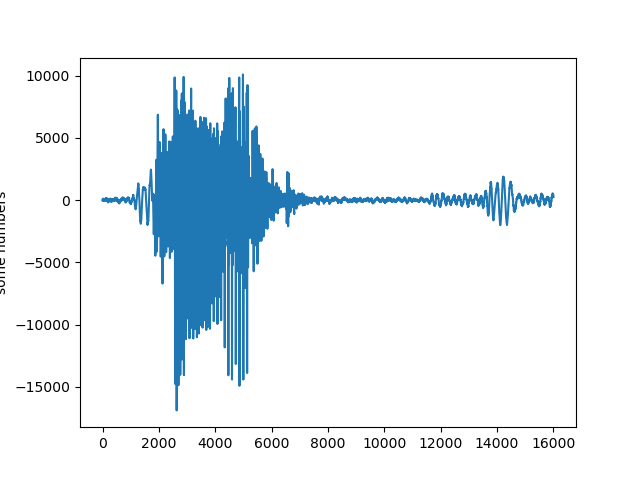
\includegraphics[width=.5\textwidth]{img/bed_rawsignal_plot.png}
	\caption{Raw signal of the \textit{bad} utterance}
	\label{fig:bed_rawsignal}
\end{figure}


\begin{figure}
	\centering
	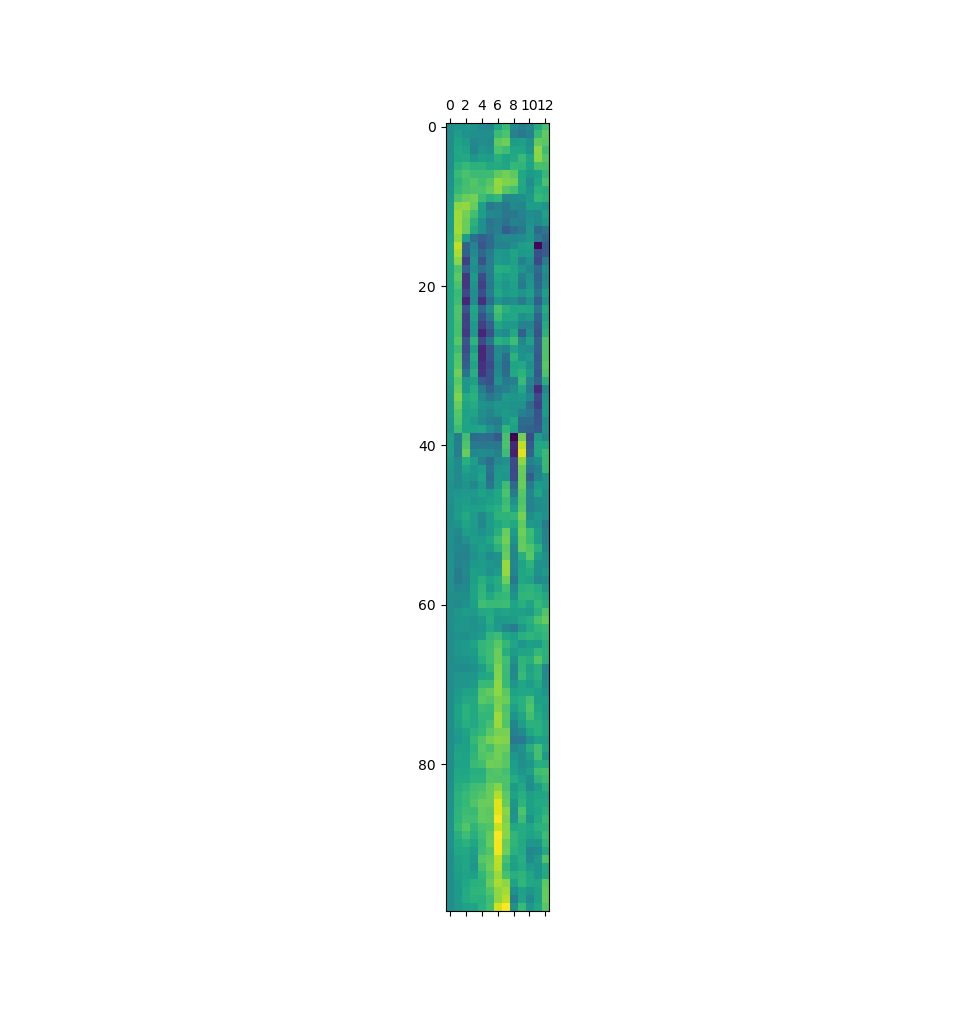
\includegraphics[width=0.5\textwidth]{img/bed_mfcc_plot.png}
	\caption{MFCC of the \textit{bad} utterance}
	\label{fig:bed_mfcc}
\end{figure}


\begin{figure}
	\centering
	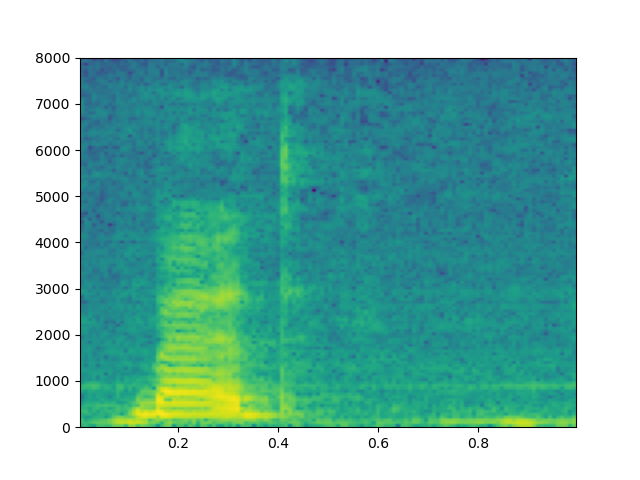
\includegraphics[width=0.5\textwidth]{img/bed_specgram_matplotlib.png}
	\caption{Spectrogram of the \textit{bad} utterance}
	\label{fig:bed_specgram}
\end{figure}


\section{Learning Framework}
\label{sec:learning_framework}

\subsection*{\textbf {CNN architectures and training}}Processed input data contain at this point the feature vectors ready to fed as input to the model. Different model structure has been analyzed using the convolutional layer as kernel of the neural network. Here there is a description of the implemented models:
\begin{itemize}
	\item \textbf{Light CNN} (light\_cnn): This is the simplest proposed model and is shown in figure \ref{fig:CNN_schema}.
	\item \textbf{Light CNN with regularization} (light\_cnn\_reg\_2): an alternative of the first model with Regularization L1\_L2 in of the weight of the first Convolutional layer.
	\item \textbf{Light CNN with Regularization and Dropout} (light\_cnn\_reg\_drop): an extension with a Dropout layer after the first Convolutional layer.
	\item \textbf{Max pool} (mp): This is an alternative of light\_cnn with a MaxPool2D after each Convolutional layer.
	\item \textbf{Double Dence} (dd): the light\_cnn with two Dence layer at the end of the sequential model.
	\item \textbf{Double Dence with Dropout} (dd\_drop): an specialized version of \textit{dd} with a Dropout layer after the first Dense layer.
\end{itemize}
\begin{figure}[h]
	\centering
	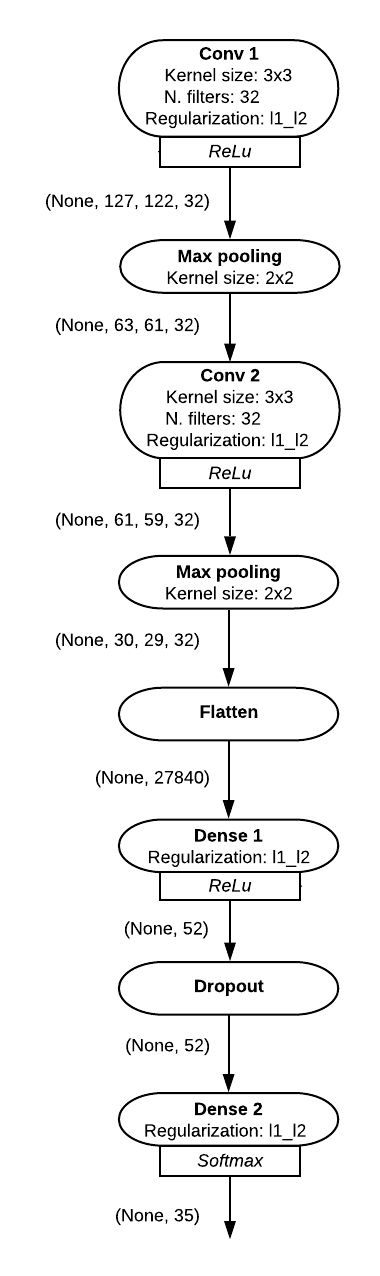
\includegraphics[width=5, height=8cm, width=0.25\textwidth]{CNN_schema}
	\caption{Light\_cnn model}
	\label{fig:CNN_schema}
\end{figure} 
\textbf{Optimizer.} The models are trained and optimized with two different built-in optimization algorithms in order to subsequently compare the obtained results. The deployed optimizers are the classic Stochastic Gradient Descent (SGD) and the Adam algorithm. \\
\textbf{Callbacks.} During the training of the model, several callbacks are passed as input to improve the performances in a computationally smart way. The {\it{ReduceOnPlateau}} callback takes care of setting the learning rate according to the behavior of the accuracy's curve; the {\it{EarlyStopping}} callback has the purpose to stop the training process, if no significant improvement is observed for a defined number of epochs. The {\it{TensorBoard}} callback function provides an interface to show the behavior of the metrics of interest during the training.

\section{Training analysis}
In Fig. \ref{fig:CNN_loss} the behavior of the loss during the training phase is shown and in Fig.  \ref{fig:CNN_accuracy} accuracy's one is depicted.

\begin{figure}[h]
			\centering
	    	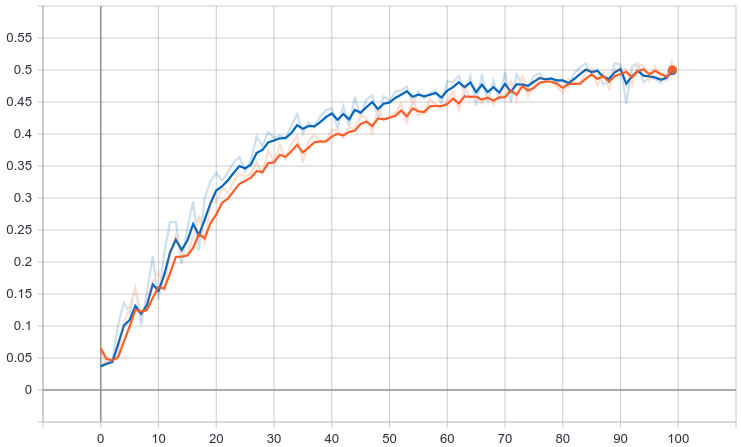
\includegraphics[width=8cm, height=6cm]{debug_tuy_acc}
	    	\caption{CNN training accuracy}
	    	\label{fig:CNN_accuracy}
\end{figure} 

\begin{figure}[h]
			\centering
	    	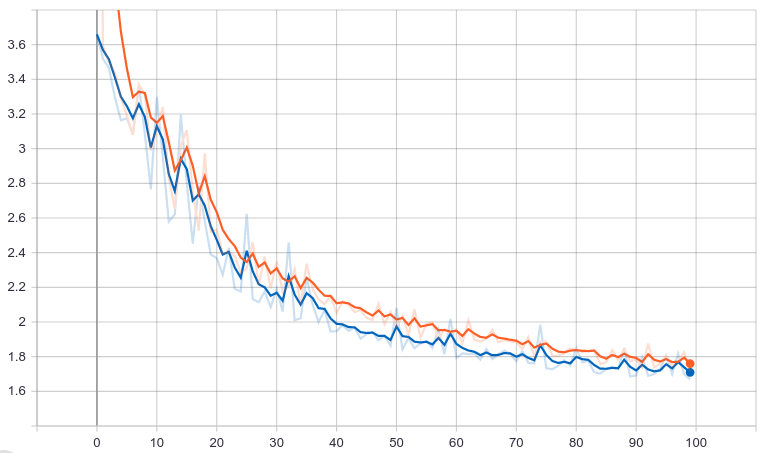
\includegraphics[width=8cm, height=6cm]{debug_tuy_loss}
	    	\caption{CNN training loss}
	    	\label{fig:CNN_loss}
\end{figure} 



